\section{Implementation}
\SectionPage

\begin{frame}
  \frametitle{Tech \sout{Heap} Stack}
  \begin{itemize}
    \item Rust, because it is a low level system language
      \pause
      \begin{itemize}
        \item Compiler knows when a value is unused
          \pause
        \item Automatically \textit{dropped}
          \pause
        \item No dangling pointers/null references
      \end{itemize}
      \pause
    \item Tauri, UI components can be created using JavaScript
      \pause
    \item Splits the core application in two, loosely coupled parts
      \begin{itemize}
        \item Frontend (JavaScript)
          \pause
        \item Backend (Rust)
      \end{itemize}
      \pause
    \item Communication is like JSON-RPC, which, effectively, is the same as a
      client-server
      \pause
    \item Allows for modules in two different languages, with little effort.
      I hoped.
  \end{itemize}
\end{frame}

\begin{frame}
  \frametitle{Blasingly Fast Memory Leakage}
  \begin{itemize}
    \item The Rust ABI is not protected by their semver notation
      \pause
    \item This means that even a patch to the Rust compiler can break a
      Rust Module
      \pause
    \item Can be fixed by using a Rust Library: \textit{abi\_stable}
      \pause
    \item Had to use `ManuallyDrop` for more complex types, which disables
      the automatic drop
      \pause
    \item Fixed by having Rust modules only reference the state, meaning
      after update and view, the module can be safely dropped
  \end{itemize}
\end{frame}

\begin{frame}
  \frametitle{I Need Super Computer Time For My Featureless App}
  \begin{itemize}
      \pause
    \item JavaScript is more \textit{unsafe} than Rust, due of a lack of typing
      \pause
    \item Need to decode the output from the modules, and catch any exceptions
      \pause
    \item When implementing the init to update to view - cycle, I tested with
      a \textit{basic} module, which should only display "Hello, World!"
      \begin{itemize}
          \pause
        \item The module initialized the state
          \pause
        \item It rendered the view
          \pause
        \item Somehow triggered an update
          \pause
        \item Which triggered a re-render
          \pause
        \item Which triggered an update
          \pause
        \item Which triggered a re-render
          \pause
        \item \dots
      \end{itemize}
  \end{itemize}
\end{frame}

\begin{frame}
  \frametitle{I Need Super Computer Time For My Featureless App}
  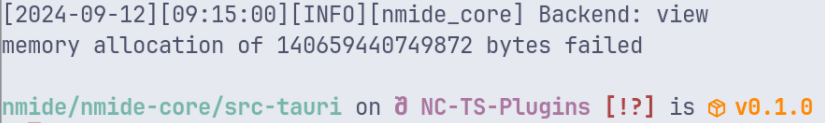
\includegraphics[width=0.9\textwidth]{./pics/memory-allocation-zoomed.png}
\end{frame}

\begin{frame}
  \frametitle{Dropped Features}
  \begin{itemize}
      \pause
    \item Language Agnostic
      \pause
    \item CI-CD
  \end{itemize}
\end{frame}
